\section*{CHAPTER 2:  DESIGN AND IMPLEMENTATION}
\addcontentsline{toc}{section}{\numberline{}CHAPTER 2: DESIGN AND IMPLEMENTATION}
\setcounter{section}{2}
\setcounter{subsection}{0}
\setcounter{figure}{0}
\setcounter{table}{0}

\subsection{OFDM Modulation method}
OFDM modulation is based on the FDM technique, with the key distinction that the subcarrier waves are placed orthogonally to each other. With this orthogonality, their signal spectra overlap without affecting the demodulation process at the receiver. The signal spectrum of a system of subcarrier waves is illustrated in Figure \ref{Spectrum} \cite{b6}.

\begin{figure}[htbp]
    \centering
    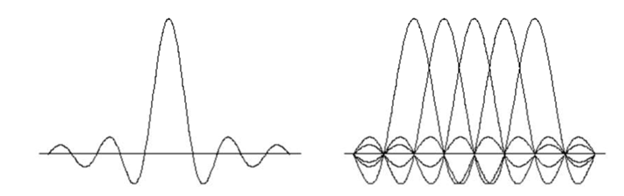
\includegraphics[width=\textwidth]{Figures/Spectrum}
    \caption{Spectrum of a single subcarrier (left) and 5 subcarriers (right)}
    \label{Spectrum}
\end{figure}

As shown in Figure \ref{Spectrum} \cite{OFDM2010}, the signal spectrum of each subcarrier channel has the form of $\frac{sin(x)}{x}$. The subcarriers are distributed evenly across the frequency range, ensuring that the peak points of one channel coincide with the null points of adjacent subcarrier channels. In the OFDM system, the signals, after passing through the digital modulator, undergo an Inverse Fast Fourier Transform (IFFT) to form OFDM symbols. The use of IFFT allows the OFDM modulator to simultaneously modulate multiple channels, a task that is challenging with FDM modulators.

\subsection{OFDM system architechure}
Figure \ref{diagram} shows a block diagram of our generic OFDM system.

\begin{figure}[htbp]
    \centering
    \documentclass[preview]{standalone}

\usepackage[english]{babel}
\usepackage{amsmath}
\usepackage{amssymb}
\usepackage[f]{esvect}
\usepackage{tikz}

\begin{document}

\usetikzlibrary{positioning}
\tikzset{block/.style={draw,thick,minimum width=1cm,minimum height=1cm,align=center}}
\tikzset{node distance=0.5cm}
\tikzset{double distance=1pt}
\tikzset{>=latex}

\begin{tikzpicture}
    \begin{scope}
        \draw [->] (-0.5,0) node [left] {$\vec{b}$}  -- (0,0) node (SP1) [right,block] {S2P};
        \node (M) [block,right=of SP1] {Mapping};
        \node (IFFT) [block,right=of M] {IFFT};
        \node (PS1) [block,right=of IFFT] {P2S};
        \node (CP) [block,right=of PS1] {Add CP};

        \draw [double,->] (PS1) -- (CP);

        \def\lines{
        \draw \ls ([yshift=3.mm]\from.east) -- ([yshift=3.mm]\to.west);
        \draw \ls ([yshift=1.mm]\from.east) -- ([yshift=1.mm]\to.west);
        \draw \ls ([yshift=-1.mm]\from.east) -- ([yshift=-1.mm]\to.west);
        \draw \ls ([yshift=-3.mm]\from.east) -- ([yshift=-3.mm]\to.west);
        }

        \def\ls{[->]}
        \def\from{SP1} \def\to{M} \lines
        \def\ls{[->,double]}
        \def\from{M} \def\to{IFFT} \lines
        \def\from{IFFT} \def\to{PS1} \lines

        \node (C) [block,below right=of CP] {Channel};

        \node (CP1) [block,below left=of C] {Remove CP};
        \node (SP2) [block,left=of CP1] {S2P};
        \node (FFT) [block,left=of SP2] {FFT};
        \node (EQ) [block,left=of FFT] {Equalize};
        \node (CE) [block,below=of EQ] {Channel\\Estimate};
        \node (Dem) [block,left=of EQ] {Demapping};
        \node (PS2) [block,left=of Dem] {P2S};
        \draw [->] (PS2.west) -- +(-0.5,0) node [left] {$\hat{b}$};

        \def\ls{[<-,double]}
        \def\from{SP2} \def\to{CP1} \lines
        \def\from{FFT} \def\to{SP2} \lines
        \def\from{EQ} \def\to{FFT} \lines
        \def\from{Dem} \def\to{EQ} \lines
        \def\ls{[<-]}
        \def\from{PS2} \def\to{Dem} \lines

        \draw [->,double,thick] (FFT.south) |- (CE.east);
        \draw [->,double,thick] (CE.north) -- (EQ.south);

        \draw [->,double] (CP) -| (C);
        \draw [->,double] (C) |- (CP1);
    \end{scope}
\end{tikzpicture}

\end{document}

    \caption{Block diagram of the OFDM system}
    \label{diagram}
\end{figure}

Principles of operation for each block:
\begin{itemize}
    \item S2P (Serial to Parallel): Converts serial data into parallel data, splitting high-speed bit streams into K lower-speed bit streams, where K is the number of subcarrier waves in the system.
    \item Mapping: QAM modulation to map pairs of bits into complex-valued constellation symbols according to the mapping\_table.
    \item IFFT(Inverse Fast Fourier Transform): Performs a fast implementation of the Inverse Discrete Fourier Transform, transforming signals from the time domain to the frequency domain, creating orthogonal subcarrier waves.
    \item P2S (Parallel to Serial): Converts parallel data back to serial, returning the signal stream to its original continuous form for transmission.
    \item Add CP:  This operation concatenates a copy of the last CP samples of the OFDM time domain signal to the beginning. This way, a cyclic extension is achieved.
    \item Channel: The wireless channel between transmitter and receiver. Here, we use a simple two-tap multipath channel.
    \item Remove CP: Remove `CP` from the received signal.
    \item FFT(Fast Fourier Transform): Transforming signals from the frequency domain to the time domain.
    \item Channel Estimate: Based on pilot signals, the receiver estimates the transmission channel using estimation algorithms.
    \item Equalize: For each subcarrier, the influence of the channel is removed such that we get the clear (only noisy) constellation symbols back.
    \item Demapping: Transform the constellation points to the pairs of bits according to the demapping\_table. The demapping table is simply the inverse mapping of the mapping\_table.
\end{itemize}